\section{Introduction}
\label{sec:background}

About 4 pages that introduces in (sufficient) depth the key concepts
and architecture of the technology.  May use a running example to
introduce the technology.

This part and other parts of the report probably needs to refer to
figures. Figure~\ref{fig:framework} from \cite{brown:96} just
illustrates how figure can be included in the report.

\begin{figure}
  \centering
  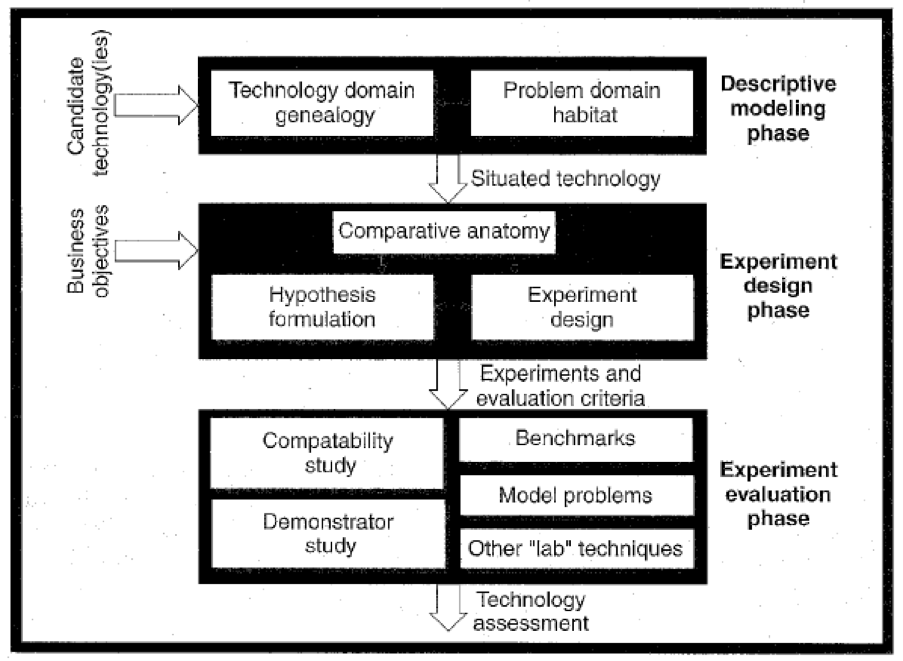
\includegraphics[scale=0.5]{figs/framework.png}
  \caption{Software technology evaluation framework.}
  \label{fig:framework}
\end{figure}


\subsection{Motivation}
we are a motivated lot ,';j

\subsection{Kotlin}

\subsubsection{What is Kotlin?}
Kotlin is a new and open source programming language. It is statically typed programming language that combines object oriented programming with functional programming. That means that one can use both styles of programming interchangeably. Kotlin comes from from JetBrains, the folk behind world's best IDE's. That means it comes from the industry and not academia so it focuses on solving some of the day-to-day tasks developers have to deal with. Kotlin is concise - which means one can expect to reduce amount of code lines written. Safe - it avoids errors like null pointer exceptions. Interoperable - use existing libraries for JVM, Android and the browser. Kotlin compiles down to JVM and Javascript which means that the language can be used for many purposes. Kotlin is also tool-friendly, one can pick any Java IDE or build directly from command line.
\subsubsection{History}
\subsubsection{Functionality} 
\paragraph{•}
\textbf{Expressiveness} - Kotlin's support for type safe builders and delegated properties help to build easy to user abstractions. \paragraph{•}
\textbf{Scalability} - Because of Kotlin's coroutines server side applications can be scaled with minimal hardware requirements. Coroutines suspend computations in a thread without blocking it. Thread blockage is often expensive, with coroutines a library can decide whether to suspend a computation or not. \paragraph{•}
\textbf{Interoperability} - Kotlin is compatible with all frameworks that work with Java. This is great because it lets developers use familiar technology while having the benefits of a modern language. \paragraph{•}
\textbf{Migration}- One can start using Kotlin and still keep older Java codebases. \paragraph{•}
\textbf{Compatibility} - Kotlin is fully compatible with JDK 6. This ensures that it can run on older android devices for example. \paragraph{}
\textbf{Performance} - Kotlin applications run just as fast as Java due to compiling to the same bytecode. Due to inline functions and code using lambdas it runs faster than code written in Java.  
\subsubsection{Where to use Kotlin}
Kotlin is great for server-side applications because of its many functionalities as mentioned in 1.2.3. \paragraph{•}
Kotlin can be used for Android development, it introduces new features while avoiding new restrictions that usually come when introducing a new technology. \paragraph{•}
JavaScript can be targeted by Kotlin and one can also use third party libraries such as JQuery and ReactJS. \paragraph{•}
Kotlin/Native is in undergoing development where compiling Kotlin to Native libraries will not require a VM. \paragraph{•}


\subsection{Kotlin Syntax}
 -On the Syntax of Kotlin (some examples)
 



